\chapter{研究内容}
\label{chap:contents}

本章では、本研究の内容を説明する。

\section{システム概要}

本システムの目的はあらゆる情報を容易に取得することだ。
サーバーは各種APIなどを用いてユーザーが必要とする情報を取得しLinda\footnote{http://linda.masuilab.org\\データをクラウド上で共有するためのフレームワーク。並列処理で同時に多くのクライアントを処理できる。}へと書き込み、Androidクライアントからのリクエストに応じてLindaからデータを取得しJSON形式でレスポンスを返す。
Androidクライアントはユーザーの操作に応じてサーバーにリクエストを送り、サーバーから返されたJSONをパースして表示する。

以下にシステムの構成を示す。

\begin{table}[htbp]
  \caption{システム構成}
  \label{tb:files}
  \begin{center}\begin{tabular}{c|l}
    \hline
    システム&概要\\\hline\hline
    {\tt Linda}&データ元。データストリームからデータを取得する。\\\hline
    {\tt サーバー}&Lindaからデータを取得し、クライアントからのリクエストが来たら送信する。\\
                      &Lindaにデータを書き込む。\\\hline
    {\tt WEBクライアント}&取得する情報を選択する為のビューを提供する。\\\hline
    {\tt Androidクライアント}&サーバーにデータを要求し、ユーザーに情報を表示する。\\\hline
    {\tt データベース}&サーバーのデータを保存している。\\\hline
  \end{tabular}\end{center}
\end{table}

\subsection{データの取得と記録}
データの取得方法としては大きく分けて三つ存在する。

まず一つ目として既存のAPIを用いて取得する方法である。天気予報や株価の情報など比較的ポピュラーな情報であれば既にAPIが存在するので、それらを用いて定期的にデータを取得しLindaへと書きこむ。

二つ目はAPIが存在しないWebページ上の情報である。例として自分の利用する公共交通機関の運行情報や特定の商品の在庫情報などである。これらのデータはKimono\footnote{https://www.kimonolabs.com/\\指定したWebページをスクレイピングし、API化するサービス。}を用いて取得したい部分のAPIを作成しデータを取得する。

三つ目はセンシングデータである。自室などに設置した各種センサーからのデータに関してはセンシングする機器から直接Lindaに書き込み、それを利用するか、もしくはサーバーで受け取ったデータを受け取りサーバーがLindaに書き込むという手法で対応する。

\subsection{ユーザーが受け取るデータの選択}

ユーザーは受け取りたい情報をWebページ上から指定する。Lindaサーバーに存在するデータの中からTupleNameとTupleTypeを指定する。(図\ref{fig:select})

\begin{figure}[htbp]
  \begin{minipage}{\hsize}
    \begin{center}
      \fbox{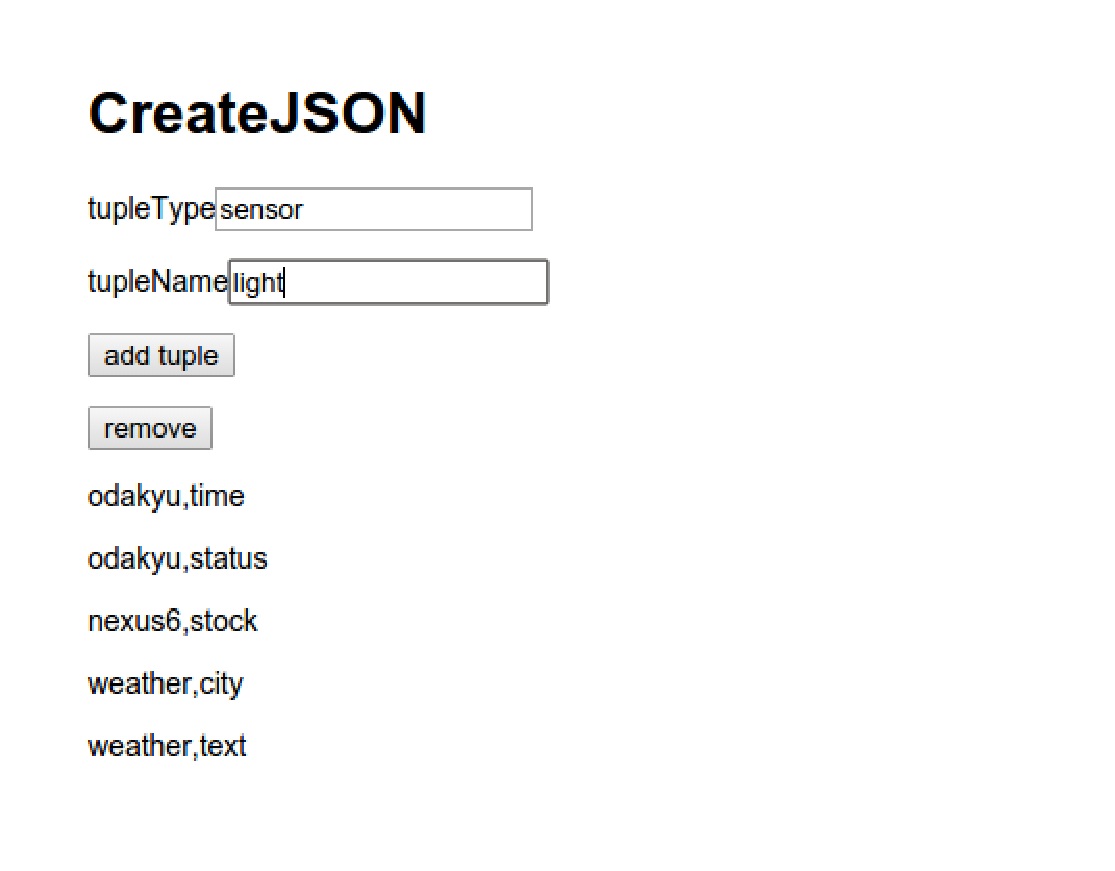
\includegraphics[width=100mm]{image/select.eps}}
    \end{center}
    \caption{Androidクライアントに送信するデータの選択}
    \label{fig:select}
  \end{minipage}
\end{figure}

\subsection{ユーザーへの情報の提供}
ユーザーが選択した情報はサーバーによって取得されJSON形式でAndroid端末へと送られる。(図\ref{fig:JSON})Androidは受け取ったJSONをパースしAndroid Widgetとして表示する。(図\ref{fig:widget})

サーバーへのリクエストはAndroid Widgetが行う自動更新、もしくはユーザーが任意のタイミングでAndroid Widgetをタップすることで行われる。

\begin{figure}[htbp]
  \begin{minipage}{\hsize}
    \begin{center}
      \begin{lstlisting}[basicstyle=\ttfamily\footnotesize, frame=single]

      {
          "info": [
              {
                  "0": "2015年01月16日14時43分現在",
                  "1": "小田急線は平常どおり運転しております。",
                  "2": "We are out of inventory. Please check back soon.",
                  "3": "Fujisawa-shi",
                  "4": "Mostly Cloudy"
              }
          ]
      }

      \end{lstlisting}
    \end{center}
    \caption{サーバーから送られるJSON}
    \label{fig:JSON}
  \end{minipage}
\end{figure}

\begin{figure}[htbp]
  \begin{minipage}{\hsize}
    \begin{center}
      \fbox{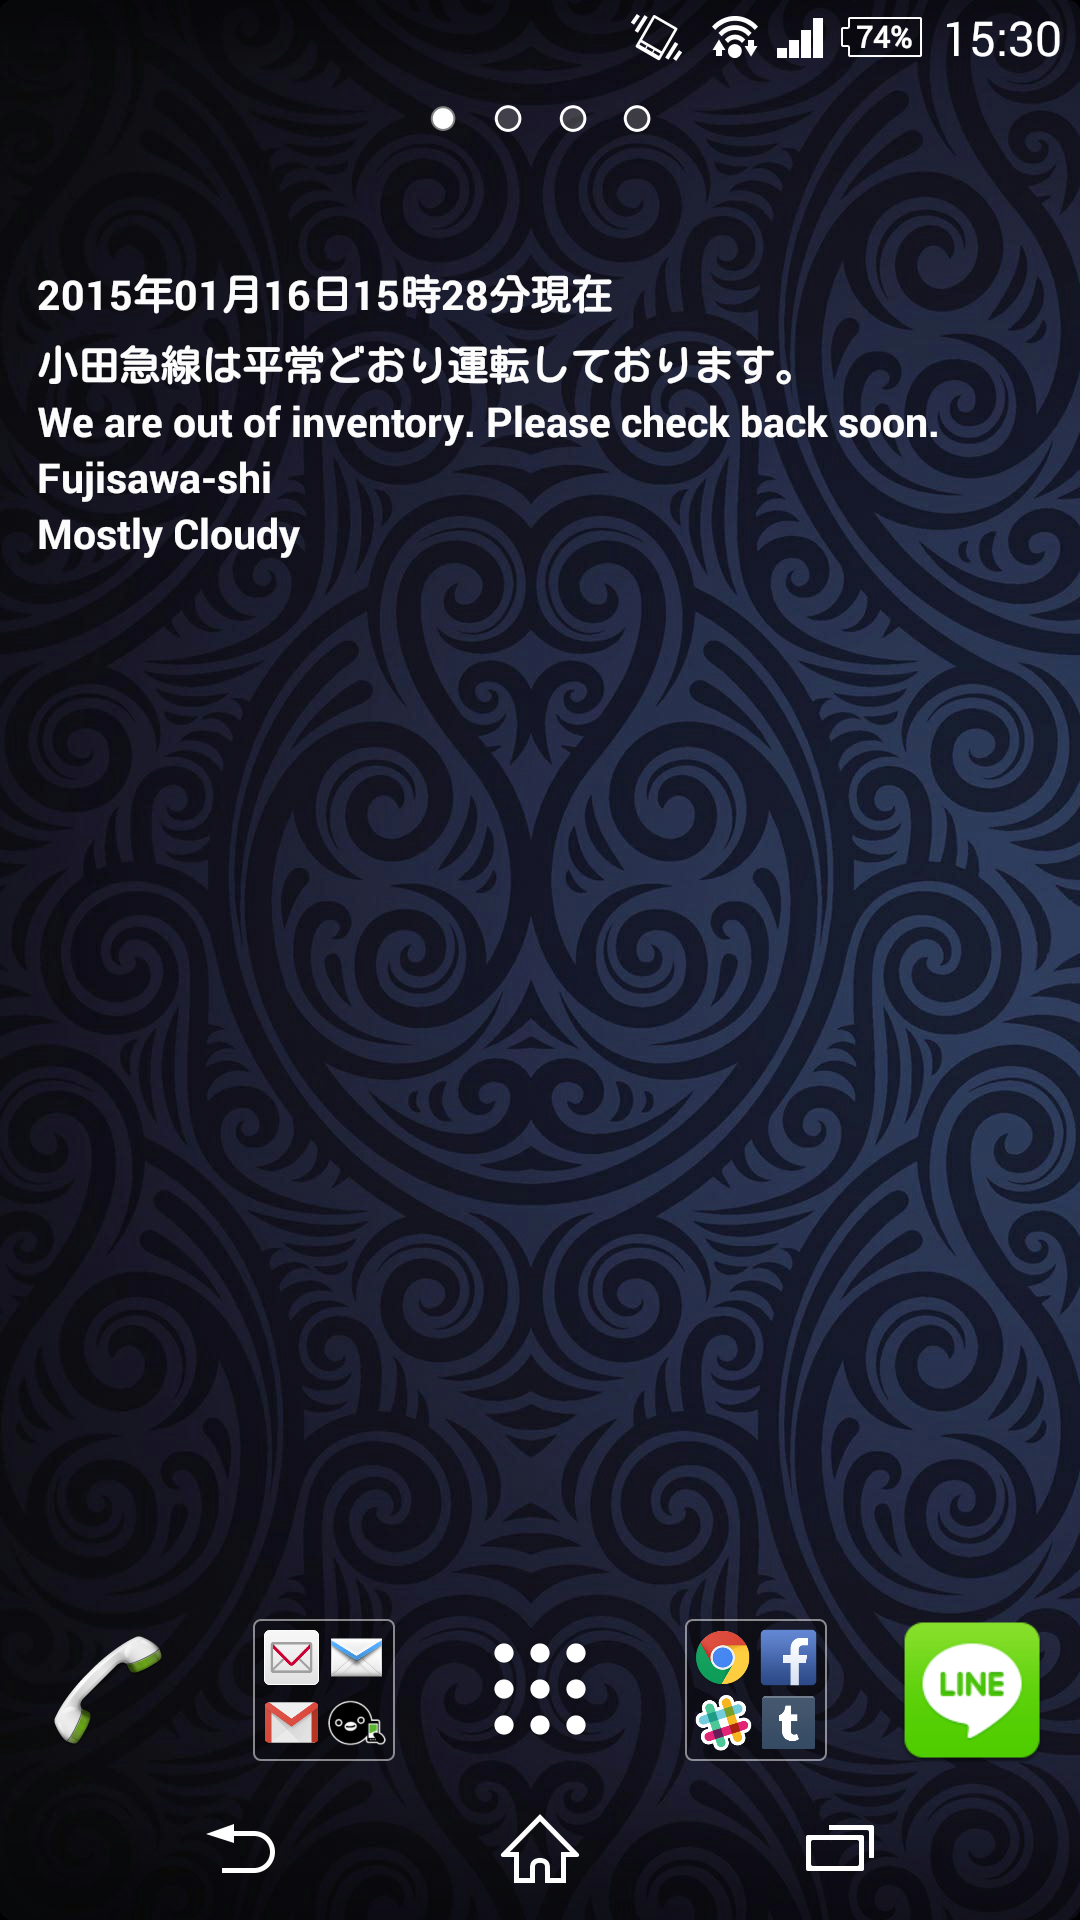
\includegraphics[width=100mm]{image/widget_single.eps}}
    \end{center}
    \caption{Android Widgetとして表示}
    \label{fig:widget}
  \end{minipage}
\end{figure}

\nocite{*}
